\subsubsection{The Word Count Problem}
\label{subsec:wcountproblem}
The Count-Distinct or Word Count Problem can be formulated as follows: given a sequence of elements $s_{1}, ..., s_{n}$ compute the amount of \textbf{distinct} elements in it. For example, for the sequence dog, cat, dog, bird, bird the answer is 3 (the distinct elements are bird, cat, and dog).

If the sequence is not too large this problem can be easily solved in expected linear time and space using hash tables, or $\mathcal{O}(nlogn)$ time and linear space using some data structures as Red-Black trees. However, this bound on space starts to become unacceptable when datasets are too large. During the last years computer scientists have managed to devise algorithms that are capable to compute approximations of the cardinality of big datasets using a constant or logarithmic amount of memory. In this project we revise a cardinality estimation algorithm name HyperLogLog \cite{Flajolet07hyperloglog:the}.\\
\\
This algorithm is very simple and yet very powerful. The core idea is the following: for each element $s_{i}$ of our sequence, use a hash function $h: \{0, 1\}^{*} \mapsto \{0, 1\}^b$ to compute a value $h(s_{i})$ and estimate the cardinality as $2^m$, where $m$ is the maximum number of leading zeros among all $h(s_{i})$. We must note that if all $h(x)$ have the same probability $\frac{1}{2^{b}}$ then the probability for some value to have $k$ leading zeros is $2^{-k}$. This means that the expected number of observations that are needed to find a number with $k$ leading zeros is $2^{k}$.\\
\\
There are some observations to be made: we need our hash function to produce at least $\log_{2}{n}$ bits, all $h(x)$ must have the same probability, and we can only answer with numbers of the form $2^{k}$. The number of bits, usually 64 \cite{40671}, is not (still) an issue, as $2^{64}$ is (still) a very big number. We also know a lot of reliable hash functions for this purpose. So our problem now is all about the limited set of answers we can give. We must note that this problem also introduces great error bounds. For example, if the answer is $\frac{2^k + 2^{k+1}}{2}$ for some $k$ then the absolute error will be at least $2^{k - 1}$.\\
\\
An interesting observation is that the function $f(\alpha) = (1 - \alpha)2^{k - 1} + \alpha2^{k}$, for $0 \leq \alpha \leq 1$ can give any value that lies in the interval $[2^{k - 1}, 2^{k}]$. We can exploit this fact to get more approximated estimations. The first idea that can come to our mind is to run various HyperLogLog with different hash functions and return the mean of all the estimations as the answer. However, it is computationally expensive to compute various different hash functions for a same token. What is done, however, is the following: 
\begin{enumerate}
\item Given a token $t$, compute $h(t)$
\item Take the first $p$ bits and use them to refer to a position in an array consisting of $2^p$ elements $a_{0}, ..., a_{2^p - 1}$
\item Update this position according to the other $b - p$ bits so it keeps the maximum amount of leading zeros seen so far
\item Once all tokens are processed output the harmonic mean of $2^{a_{0}}, ..., 2^{a_{2^p - 1}}$ as the answer.
\end{enumerate}
This approach, known as HyperLogLog \cite{Flajolet07hyperloglog:the}, still requires a single pass and still requires only one hash function to work. If we use 64 bits (as HyperLogLog++ \cite{40671} does) as the size of the image of our hash function and 14 bits as the index in our array we will have $2^{14} = 16384$ different records while still being capable to estimate datasets with cardinality $2^{50} = 1125899906842624 > 10^{15}$, so it does not seem that this should make us worry about not having enough bits\footnote{https://github.com/antirez/redis/blob/unstable/src/hyperloglog.c}.\\
\\
An interesting trivia fact is that if we need $\mathcal{O}(\log n)$ bits for our hash function to be able to count until $n$ then we only need $\mathcal{O}(\log \log n)$ to store the number of leading zeros of some hash value. This is why HyperLogLog is called that way.\\
\\
A very nice property of HyperLogLog is that two distinct runs on two different datasets can be merged if they have used the same parameters (hash function, $b$, and $p$) in such a way that it approximates the cardinality of the union of the two datasets. Given two arrays $a$ and $b$, each corresponding to a run of HyperLogLog we can get a fictional run of HyperLogLog $c$ that represents the union of both datasets by computing $c_{i} =\max(a_{i}, b_{i})$ for all of the $2^{p}$ positions. This makes sense, as it produces the same result as running a single HyperLogLog on the concatenation of the two datasets. This property allows us to parallelize or to distribute this algorithm, giving us a potential performance boost. The source code we will use for our experiments is the following:
\newpage
\inputminted{python}{applications/HYPERLOGLOG/main.py}
The \verb|HyperLogLog| class can be found in the project's GitHub repository\footnote{https://github.com/srgrr/TFM/blob/master/applications/HYPERLOGLOG/main.py}.
Note that this application is a classical \textit{map-reduce} workflow. Without collections we are forced to implement any reduce function as \verb|reduce(f, *args)|. Each extra argument is passed as an input parameter via socket and pipe, implying a huge overhead. With collections only the collection object, and the list of identifiers, are transferred. The other properties of the contents, such as direction, locations and so on, are deduced or requested in the destination node.\\
\\
The elimination of this overhead is noticeable even with a very small number of parameters. As we can see in figure \ref{fig:collection_vs_normal}, the collection feature reduces the overhead drastically. An important observation is that a PyCOMPSs task of the form \verb|f(*args)| usually starts to show problems and crashes when more than $60$ arguments are passed, as each argument represents a lot of metadata to be transferred via socket and pipe.
\begin{figure}[ht!]
\centering
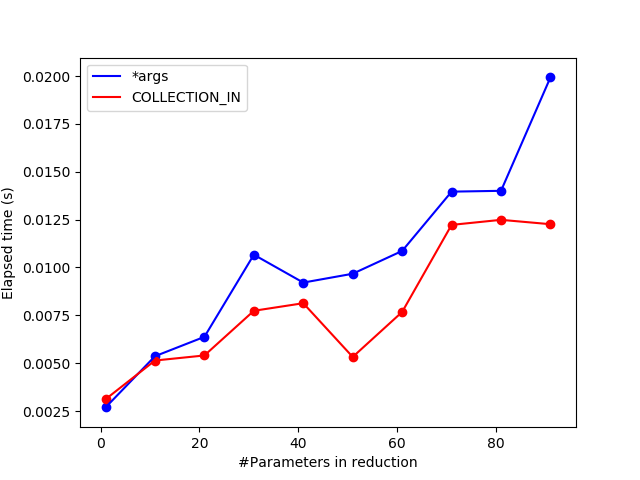
\includegraphics[scale = 0.5]{figures/collection_vs_normal.png}
\caption{Execution time of the reduce functions with and without collections. Each point is the average of 5 executions. Although the samples are noisy, as they are small, a consistent improvement by the collection feature can be appreciated. The non-collections versions started to crash and to show strange behaviours around the 60 parameters}
\label{fig:collection_vs_normal}
\end{figure}\\
\\
Let's note that for a task \verb|f(a, b, c, d, e)| the following information is sent through a socket:

\begin{verbatim}
[BINDING-COMMONS]  -  @GS_RegisterCE  -  Task registered: metadata.f
[BINDING-COMMONS]  -  @GS_ExecuteTaskNew - Processing task execution in bindings-common. 
[BINDING-COMMONS]  -  @GS_ExecuteTaskNew  -  Processing parameter 0
[BINDING_COMMONS]  -  @process_param
[BINDING-COMMONS]  -  @process_param  -  ENUM DATA_TYPE: 9
[BINDING-COMMONS]  -  @process_param  -  File: ...
[BINDING-COMMONS]  -  @process_param  -  ENUM DIRECTION: 0
[BINDING-COMMONS]  -  @process_param  -  ENUM STREAM: 3
[BINDING-COMMONS]  -  @process_param  -  PREFIX: null
[BINDING-COMMONS]  -  @process_param  -  NAME: *args*_0
[BINDING-COMMONS]  -  @GS_ExecuteTaskNew  -  Processing parameter 1
[BINDING_COMMONS]  -  @process_param
[BINDING-COMMONS]  -  @process_param  -  ENUM DATA_TYPE: 9
[BINDING-COMMONS]  -  @process_param  -  File: ...
[BINDING-COMMONS]  -  @process_param  -  ENUM DIRECTION: 0
[BINDING-COMMONS]  -  @process_param  -  ENUM STREAM: 3
[BINDING-COMMONS]  -  @process_param  -  PREFIX: null
[BINDING-COMMONS]  -  @process_param  -  NAME: *args*_1
[BINDING-COMMONS]  -  @GS_ExecuteTaskNew  -  Processing parameter 2
[BINDING_COMMONS]  -  @process_param
[BINDING-COMMONS]  -  @process_param  -  ENUM DATA_TYPE: 9
[BINDING-COMMONS]  -  @process_param  -  File: ...
[BINDING-COMMONS]  -  @process_param  -  ENUM DIRECTION: 0
[BINDING-COMMONS]  -  @process_param  -  ENUM STREAM: 3
[BINDING-COMMONS]  -  @process_param  -  PREFIX: null
[BINDING-COMMONS]  -  @process_param  -  NAME: *args*_2
[BINDING-COMMONS]  -  @GS_ExecuteTaskNew  -  Processing parameter 3
[BINDING_COMMONS]  -  @process_param
[BINDING-COMMONS]  -  @process_param  -  ENUM DATA_TYPE: 9
[BINDING-COMMONS]  -  @process_param  -  File: ...
[BINDING-COMMONS]  -  @process_param  -  ENUM DIRECTION: 0
[BINDING-COMMONS]  -  @process_param  -  ENUM STREAM: 3
[BINDING-COMMONS]  -  @process_param  -  PREFIX: null
[BINDING-COMMONS]  -  @process_param  -  NAME: *args*_3
[BINDING-COMMONS]  -  @GS_ExecuteTaskNew  -  Processing parameter 4
[BINDING_COMMONS]  -  @process_param
[BINDING-COMMONS]  -  @process_param  -  ENUM DATA_TYPE: 9
[BINDING-COMMONS]  -  @process_param  -  File: ...
[BINDING-COMMONS]  -  @process_param  -  ENUM DIRECTION: 0
[BINDING-COMMONS]  -  @process_param  -  ENUM STREAM: 3
[BINDING-COMMONS]  -  @process_param  -  PREFIX: null
[BINDING-COMMONS]  -  @process_param  -  NAME: *args*_4
[BINDING-COMMONS]  -  @GS_ExecuteTaskNew  -  Processing parameter 5
[BINDING_COMMONS]  -  @process_param
[BINDING-COMMONS]  -  @process_param  -  ENUM DATA_TYPE: 9
[BINDING-COMMONS]  -  @process_param  -  File: ...
[BINDING-COMMONS]  -  @process_param  -  ENUM DIRECTION: 1
[BINDING-COMMONS]  -  @process_param  -  ENUM STREAM: 3
[BINDING-COMMONS]  -  @process_param  -  PREFIX: #
[BINDING-COMMONS]  -  @process_param  -  NAME: $return_0
\end{verbatim}

While the collection equivalent generates this data:

\begin{verbatim}
[BINDING-COMMONS]  -  @GS_RegisterCE  -  Task registered: metadata.g
[BINDING-COMMONS]  -  @GS_ExecuteTaskNew - Processing task execution in bindings-common. 
[BINDING-COMMONS]  -  @GS_ExecuteTaskNew  -  Processing parameter 0
[BINDING_COMMONS]  -  @process_param
[BINDING-COMMONS]  -  @process_param  -  ENUM DATA_TYPE: 26
[BINDING-COMMONS]  -  @process_param  -  Collection: ...
[BINDING-COMMONS]  -  @process_param  -  ENUM DIRECTION: 0
[BINDING-COMMONS]  -  @process_param  -  ENUM STREAM: 3
[BINDING-COMMONS]  -  @process_param  -  PREFIX: null
[BINDING-COMMONS]  -  @process_param  -  NAME: c
[BINDING-COMMONS]  -  @GS_ExecuteTaskNew  -  Processing parameter 1
[BINDING_COMMONS]  -  @process_param
[BINDING-COMMONS]  -  @process_param  -  ENUM DATA_TYPE: 9
[BINDING-COMMONS]  -  @process_param  -  File: ...
[BINDING-COMMONS]  -  @process_param  -  ENUM DIRECTION: 1
[BINDING-COMMONS]  -  @process_param  -  ENUM STREAM: 3
[BINDING-COMMONS]  -  @process_param  -  PREFIX: #
[BINDING-COMMONS]  -  @process_param  -  NAME: $return_0
\end{verbatim}
